\documentclass[12pt, a4paper]{report}
\usepackage[utf8]{inputenc}
\usepackage{graphicx}
\graphicspath{{graphs/}}
\title{Implantations efficaces de calculs sur les polynômes à une variable : FFT}
\author{}
\date{7 Avril 2022}

\begin{document}
\maketitle
\tableofcontents
\newpage

\chapter*{Introduction}
\addcontentsline{toc}{chapter}{Introduction}
intro


\chapter{L'algorithme de Karatsuba}
test
\section{Partie 1}

\section{Partie 2}

\chapter{Fast Fourier Transform (FFT)}
\section{Partie 1}
\subsection{Sous partie 1.1}
\section{Partie 2}

test
image :\\
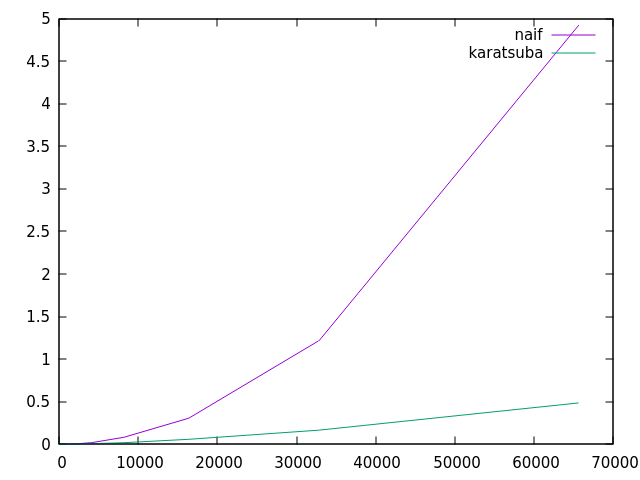
\includegraphics[scale=1]{naif_kara}\\

l'équation dans la phrase $e^{i\pi}+1 = 0$\\
l'équation au milieu numerotée
\begin{equation}
E=mc^2
\end{equation}
l'equation au mileu non numerotée
\[ E=mc^2 \]

Ceci est une liste :
\begin{enumerate}
  \item premier element
  \item deuxieme element
\end{enumerate}

\end{document}